\section{Implementation completion}

\subsection{Constraints specification}
First step to complete our implementation of the database is to complete a set of constraints, especially the referential integrity constraints of the foreign keys. Luckily, MySQLWorkbench provides us with a simple interface to set these constraints.

\begin{figure}[H]
    \centering
    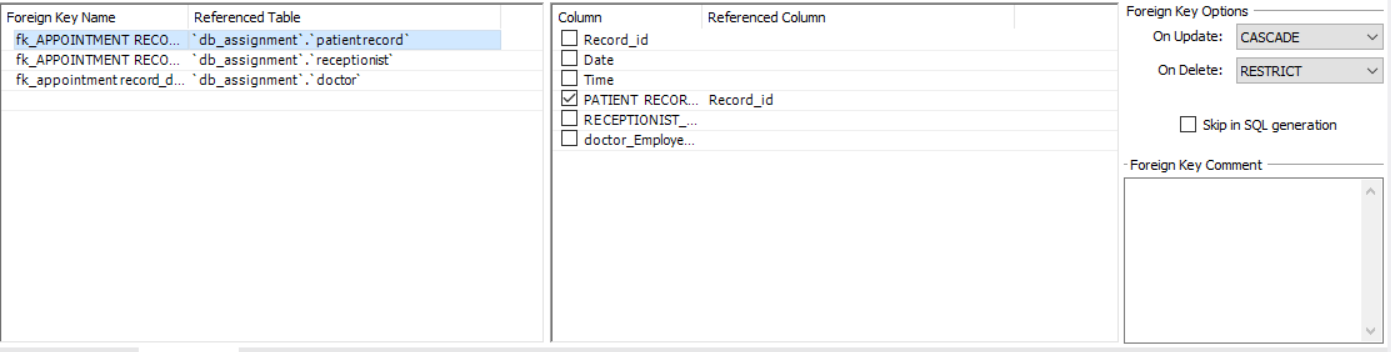
\includegraphics[width = 12cm]{assets/constraints_1.png}
    \captionsetup{justification=centering,margin=2cm}
    \caption{MySQL Workbench foreign keys options features}
\end{figure}

As we can see, the window on the right side allow us the ability to set the options when DELETE and UPDATE.We have 4 total options to choose (RESTRICT, CASCADE, SET NULL, NO ACTION). Now we will have to go through each of our foreign keys and set the suitable option.

\begin{itemize}
    \item On \textcolor{blue}{DOCTOR} table, we have 1 FK referenced to \textcolor{blue}{DEPARTMENT} table. We would set CASCADE on both ON UPDATE AND ON DELETE.The reason for this choice is due to a business rule that when a \textcolor{blue}{DEPARTMENT} is removed, every doctors should be removed as well.
    \item For the rest of our tables, we would choose CASCADE ON UPDATE and RESTRICT ON DELETE. When the referenced table UPDATE their value, it is obvious that the referencing table should UPDATE as well, so we choose CASCADE ON UPDATE. For ON DELETE options, we choose RESTRICT because when a referenced table is deleted, we don't have to delete the referencing table as well because they represents two distinct entities.
\end{itemize}

\subsection{Triggers}

\subsubsection{Trigger on Employee's Salary}
The first trigger we would like to set is a constraint on the input of Salary column in EMPLOYEE table. If a person wants to insert a negative value into our table, we would automatically set it to 0 as default.

\begin{figure}[H]
    \centering
    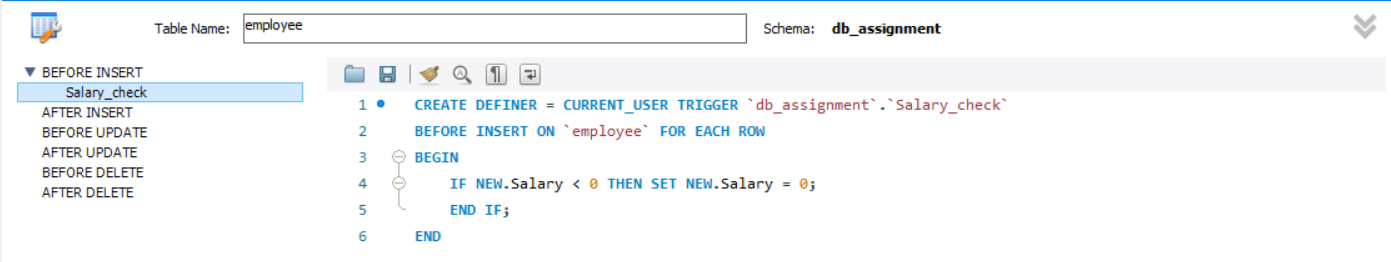
\includegraphics[width = 12cm]{assets/trigger_1.png}
    \captionsetup{justification=centering,margin=2cm}
    \caption{Trigger on Employee's Salary}
\end{figure}

\subsubsection{Trigger on Experience of NURSE}
The second trigger is similar to the first one in terms of checking BEFORE\_INSERT constraint. In this case, we would also set a default value of 0 whenever a person accidentally inserted a negative value of Experience column of NURSE table.

\begin{figure}[H]
    \centering
    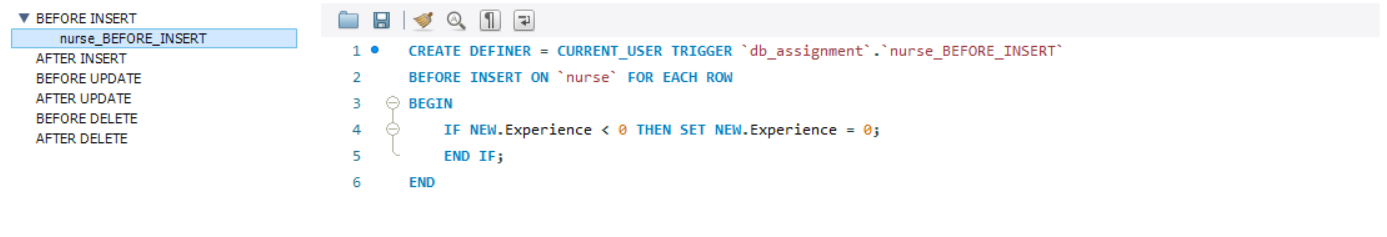
\includegraphics[width = 12cm]{assets/trigger_2.png}
    \captionsetup{justification=centering,margin=2cm}
    \caption{Trigger on Nurse's Experience}
\end{figure}

\subsubsection{Trigger on date of Appointment record}

The final trigger in our assignment is about the default value for a DATETIME type value, which is one of the most common usage of trigger. We would create a trigger to automatically set the current date in to the 

\begin{figure}[H]
    \centering
    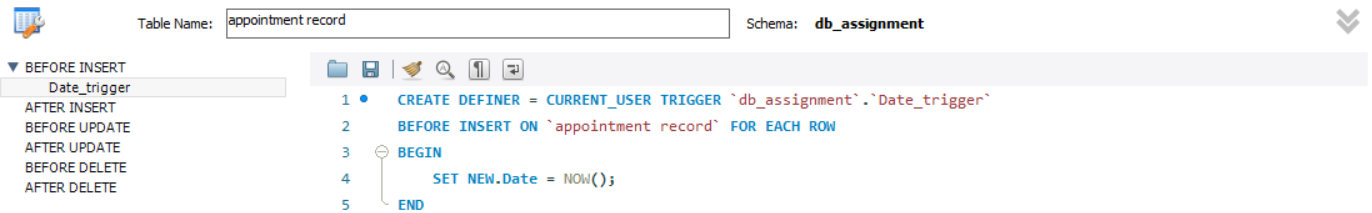
\includegraphics[width = 12cm]{assets/trigger_3.png}
    \captionsetup{justification=centering,margin=2cm}
    \caption{Trigger on Appointment Record}
\end{figure}

\subsection{Queries}

\subsubsection{Retrieve a full form of medical records}
As we mentioned earlier, one big improvement of our database after normalizing is the spilt of MEDICAL RECORD table into 2 sub tables, PATIENT PROFILE and PATIENT RECORD. However, when we want to get the information of the whole medical record, we have to join those 2 table. 

\begin{figure}[H]
    \centering
    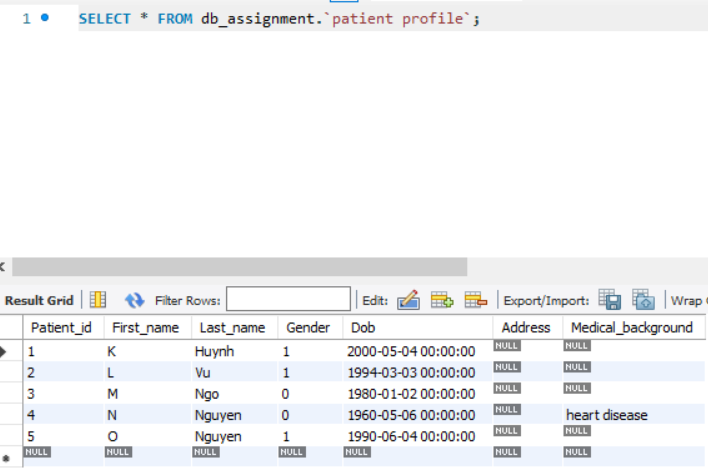
\includegraphics[width = 12cm]{assets/query_1c.png}
    \captionsetup{justification=centering,margin=2cm}
    \caption{PATIENT PROFILE table}
\end{figure}

\begin{figure}[H]
    \centering
    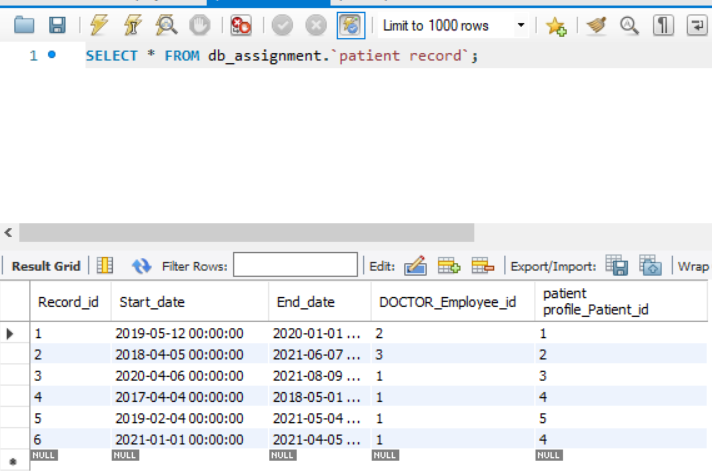
\includegraphics[width = 12cm]{assets/query_1b.png}
    \captionsetup{justification=centering,margin=2cm}
    \caption{PATIENT RECORD table}
\end{figure}

\begin{figure}[H]
    \centering
    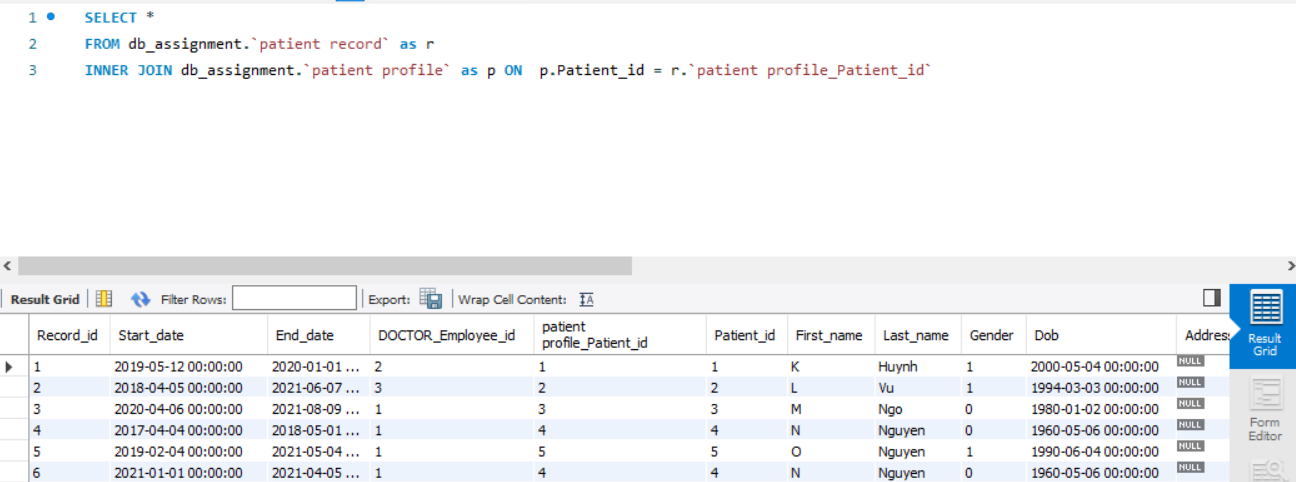
\includegraphics[width = 12cm]{assets/query_1a.png}
    \captionsetup{justification=centering,margin=2cm}
    \caption{Query and Result}
\end{figure}

As a result of the above query, we have a full form of a medical record.

\subsubsection{Get all prescriptions of patient "Nguyen N" }
In this query, we would like to retrieve all prescriptions of a patient named "Nguyen N". As we already know, patient First name and Last name is stored in the PATIENT PROFILE table.While prescriptions are stored in PRESCRIPTION table, which have a foreign key referencing to Record id of PATIENT RECORD.Therefore, we first have to lookup the Record id of patient Nguyen N, then join with Prescription table on that Record id.

\begin{figure}[H]
    \centering
    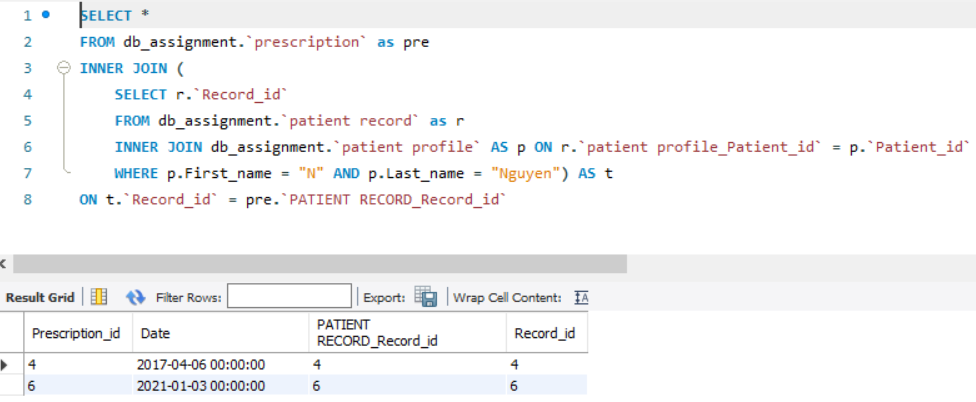
\includegraphics[width = 12cm]{assets/query_2.png}
    \captionsetup{justification=centering,margin=2cm}
    \caption{List of prescriptions used by Nguyen N}
\end{figure}

From the result we could conclude that Nguyen N has 2 prescriptions.

\subsubsection{Get the number patients treated by doctor "Nguyen A"}

For the last query, we will get the number of patients treated by doctor Nguyen A. From our database design, we know that employee names are stored in EMPLOYEE table. Therefore, we have to find the Employee id of doctor Nguyen N, then find the number of patients treated by him.

\begin{figure}[H]
    \centering
    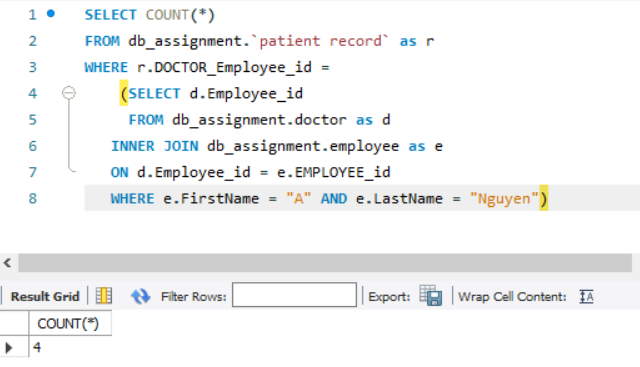
\includegraphics[width = 12cm]{assets/query_3a.png}
    \captionsetup{justification=centering,margin=2cm}
    \caption{Number of patients of doctor Nguyen A}
\end{figure}

\subsection{Stored procedures}

\subsubsection{Get monthly report of patient records}
For our first store procedure, we would like to store the query to retrieve the complete form of a medical record like the first query. Because of that, we just need to store the query above into a procedures called Get\_report.

\begin{figure}[H]
    \centering
    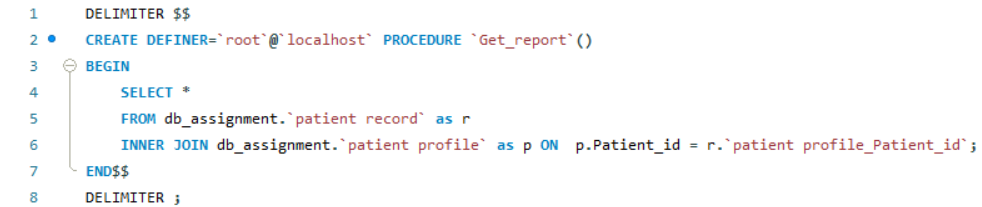
\includegraphics[width = 12cm]{assets/procedure_1a.png}
    \captionsetup{justification=centering,margin=2cm}
    \caption{Procedure creation code}
\end{figure}

\begin{figure}[H]
    \centering
    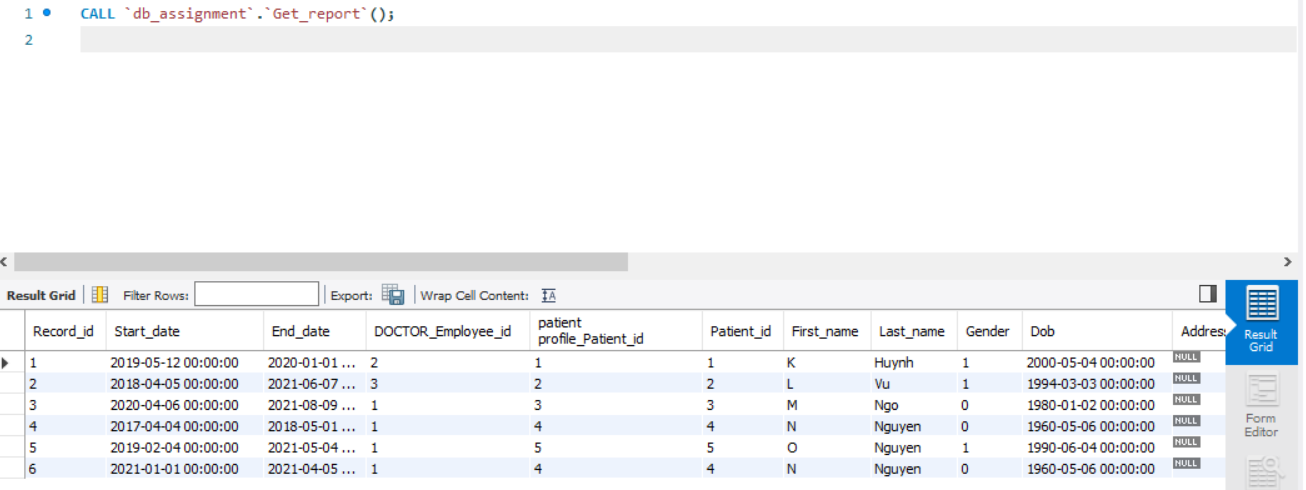
\includegraphics[width = 12cm]{assets/procedure_1b.png}
    \captionsetup{justification=centering,margin=2cm}
    \caption{Procedure call result}
\end{figure}

\subsubsection{Get number of patients stays in one department}

Next, a department would like to know how many patients have stayed in their building. Therefore we create a procedure call named Get\_number\_of\_patients to get the number of patients stays in one department.Regarding the SQL code, we have to how many patients have stayed in which rooms that belongs to which department.

\begin{figure}[H]
    \centering
    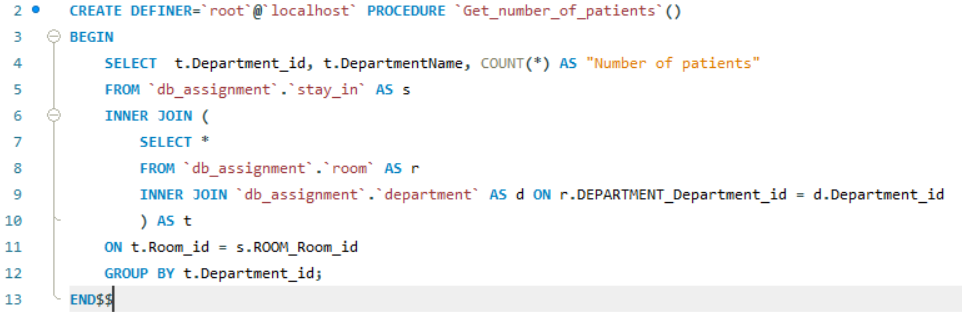
\includegraphics[width = 12cm]{assets/procedure_2a.png}
    \captionsetup{justification=centering,margin=2cm}
    \caption{Procedure creation}
\end{figure}

\begin{figure}[H]
    \centering
    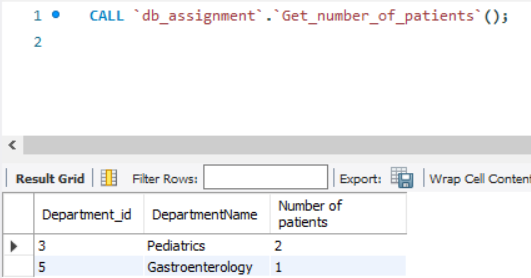
\includegraphics[width = 12cm]{assets/procedure_2b.png}
    \captionsetup{justification=centering,margin=2cm}
    \caption{Procedure call result}
\end{figure}
From the result, we could say that there are 2 patients stay in Pediatrics department and 1 patient stay in Gastroenterology department.

\subsubsection{Get a list of tests that were made by the hospital}
Last but no least, our final procedure is about getting a list of tests that were made by the hospital. We know that a hospital conducts a lot of tests. Therefore we have to get a report about all kinds of tests have been made.

\begin{figure}[H]
    \centering
    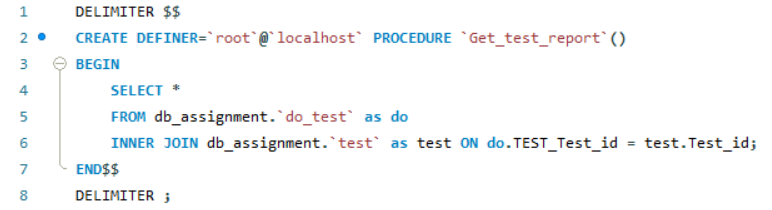
\includegraphics[width = 12cm]{assets/procedure_3a.png}
    \captionsetup{justification=centering,margin=2cm}
    \caption{Procedure call result}
\end{figure}

\begin{figure}[H]
    \centering
    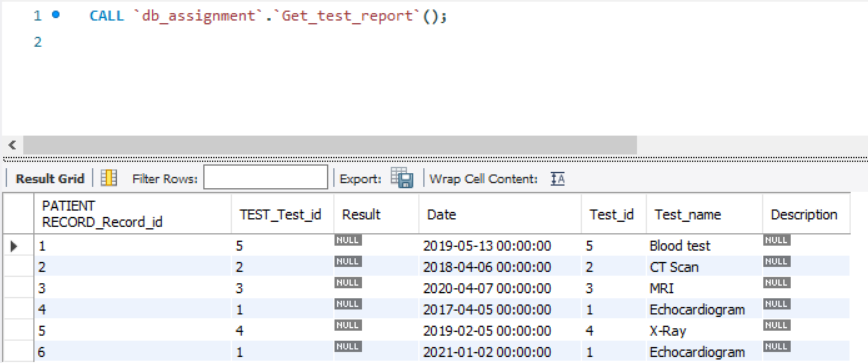
\includegraphics[width = 12cm]{assets/procedure_3b.png}
    \captionsetup{justification=centering,margin=2cm}
    \caption{Procedure call result}
\end{figure}

From our query, we could see the whole list of tests were conducted by the hospitals.